\documentclass[pdf]{beamer}
\mode<presentation>{}
\usepackage{minted}
\usepackage{tikz}
\usepackage{pgffor} %% gives looping with \foreach
\usepackage[absolute,overlay]{textpos}
\usepackage{lmodern} %% scalable latin characters
\usetikzlibrary{arrows,shapes,backgrounds}
\usepackage{multirow}
\usepackage{listings} %% another package for code related stuff

%% stuff for minted
\definecolor{mintedBg}{rgb}{0.95, 0.95, 0.95}
\definecolor{blockBg}{rgb}{0.6, 0.6, 0.95}
\definecolor{rnaColor}{rgb}{0, 0.6, 0}
\definecolor{cdsColor}{rgb}{0, 0.4, 0.4}
\definecolor{rnaPol}{rgb}{0.8,0,0.8}
\definecolor{ribosomeCol}{rgb}{0.5,0.5,0.1}
\definecolor{protColor}{rgb}{0.6,0,0.6}
%% colours for nucleotides:
\definecolor{dACol}{rgb}{0.5, 0.5, 0}
\definecolor{dCCol}{rgb}{0.8, 0, 0}
\definecolor{dGCol}{rgb}{0, 0.8, 0}
\definecolor{dTCol}{rgb}{0, 0, 0.8}

\definecolor{navy}{rgb}{0, 0, 0.6}
\definecolor{pur}{rgb}{0, 0, 0.6}
\definecolor{pyr}{rgb}{0.6, 0, 0.2}
%% define styles for different codes
\newminted{cpp}{linenos, bgcolor=blockBg, fontsize=\footnotesize}
%% then use \begin{cppcode}
\newminted{c}{linenos, bgcolor=mintedBg, fontsize=\footnotesize}
\newminted{perl}{linenos, bgcolor=mintedBg, fontsize=\footnotesize}

%% a command to define a subheading
\newcommand\subHeading[1]{
  \par\bigskip {\Large\bfseries#1}\par\smallskip
}

%% I detest indentation in footnotes etc, so try this:
\makeatletter
\renewcommand\@makefntext[1]{\noindent\makebox[0em][r]{\@makefnmark}\tiny#1}
\makeatother
%% the makeatletter and makeatother are required to allow me to
%% to change the macro beginning with an @. (though when I call it
%% I don't use the @ ... 

\setlength\parskip{0.5em}
\setlength\parindent{0ex}

%% to have footnotes without references. This from tex.stackexchange.com
\newcommand\blfootnote[1]{%
  \begingroup  %% this makes it a local redefinition
  \renewcommand\thefootnote{}\footnote{#1}%
  \addtocounter{footnote}{-1}  % this adjusts the footnote counter
  \endgroup
}


\title{Databases}
\subtitle{Structuring data}
\author{Martin Jakt}

\begin{document}

\begin{frame}
  \titlepage
\end{frame}

\begin{frame}{What is a database?}
  In its simplest form:\\
  \textcolor{navy}{A collection of data in some defined format}
  \pause
  \begin{itemize}
  \item Flat files
  \item Relational
  \item Object orientated
  \end{itemize}

  \pause
  We will be primarily concerned with relational, but first..

  \visible<2->{
    \blfootnote{There are some others as well, but these are the main types}
  }

\end{frame}

\begin{frame}{Flat files}
No specific requirements but the data in the files should follow 
some predefined specification describing the encoding and organisation
of the data.

Some examples:
\begin{description}
\item[Sequences] A collection of fasta files, or a single multisequence fasta file
\item[Expression] A collection of Soft format files
\item[Images] A collection of jpegs
\end{description}

Easy to create, difficult to query (eg. need to read all files to get all sequence names or lengths).

Good for genome sequences (but not the annotation).
\end{frame}

\begin{frame}{Object orientated}
  \begin{itemize}
  \item Data is structured into classes
  \item Objects are instances of classes
  \item Objects are collections of other objects
  \end{itemize}
\end{frame}

\begin{frame}{Object orientated}
  For example: A gene can be represented by a class that contains:
  \begin{itemize}
  \item Promoter
  \item Splice site acceptors
  \item Splice site donors
  \item polyA signal
  \item Transcripts
  \end{itemize}
  
  Where Promoter, Splice site acceptors themselves are objects of their own right.
  
  Object orientated databases are more flexible in the types of data
  that they can represent (esp. tree like) but trade off flexibility
  in querying for speed.

  Suitable for big and or complicated data-sets?
\end{frame}

\begin{frame}{Relational}
  \begin{itemize}
  \item provide a framework for storing data in a structured manner
  \item provide mechanisms for ensuring data integrity
  \item based on well understood\footnote{by discrete mathematicians} discrete mathematics
  \end{itemize}
  \pause
  But what does that mean?
\end{frame}

\begin{frame}{Typical experimental data}
%  pgfversion is \pgfversion
  \begin{figure}[ht]
    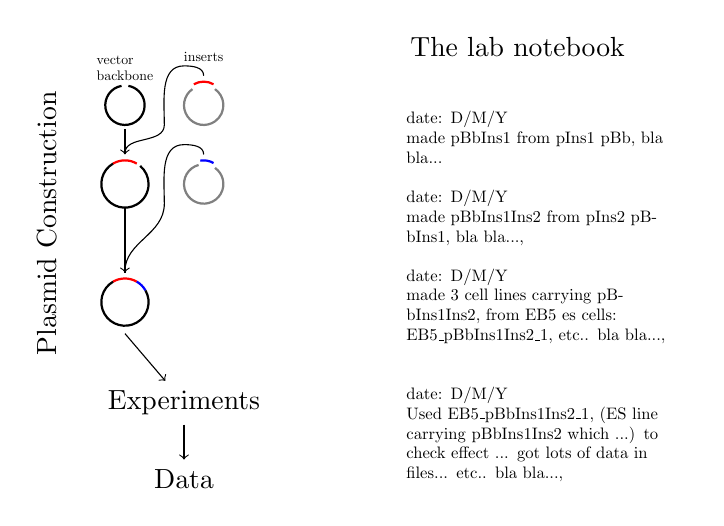
\begin{tikzpicture}[scale=0.5]
%      \draw [help lines, opacity=1] (0,0) grid (22,12);
%      \foreach \x in {1,2,...,20} \node [font=\small] at (\x,0) {\x};
%      \foreach \y in {1,2,...,11} \node [font=\small] at (20,\y) {\y};
      
      \node [above, rotate=90] at (-1.5,7) {Plasmid Construction};

      \visible<1->{
      \draw [-, black, thick] (0,10) ++(90+10:0.5) arc((90+10):(360+90-10):0.5);
      \draw [-, gray, thick] (2,10) ++(90+35:0.5) arc((90+35):(360+90-35)):0.5); 
      \draw [-, red, thick] (2,10.1) ++(90+30:0.5) arc((90+30):(90-30)):0.5); 
      
      \draw [->] (2,10.75) to [out=90,in=0] (1.5,11)
            to [out=180,in=90] (1,9.5)
            to [out=270,in=90] (0,8.75);
      \draw [-] (0,9.4) -- (0,8.75); 
      

%      \draw [-, black, thick] (1,8) ++(90+30:0.6) arc((90+30):(360+90-30)):0.6); 
%      \draw [-, red, thick] (1,8) ++(90+30:0.6) arc((90+30):(90-30)):0.6); 
      \draw [-, black, thick] (0,8) ++(90+30:0.6) arc((90+30):(360+90-40)):0.6); 
      \draw [-, red, thick] (0,8) ++(90+30:0.6) arc((90+30):(90-30)):0.6); 
      }
      \visible<2->{
      \draw [-, gray, thick] (2,8) ++(90+15:0.5) arc((90+15):(360+90-35)):0.5); 
      \draw [-, blue, thick] (2,8.1) ++(90+10:0.5) arc((90+10):(90-30)):0.5); 

      \draw [->] (2,8.75) to [out=90,in=0] (1.5,9)
            to [out=180,in=90] (1,7.5)
            to [out=270,in=90] (0,5.75);
      \draw [-] (0,7.4) -- (0,5.75); 
            
      \draw [-, black, thick] (0,5) ++(90+30:0.6) arc((90+30):(360+90-60)):0.6); 
      \draw [-, red, thick] (0,5) ++(90+30:0.6) arc((90+30):(90-30):0.6); 
      \draw [-, blue, thick] (0,5) ++(90-30:0.6) arc((90-30):(90-60):0.6); 
      }

      \node [above, align=left, scale=0.5] at (0,10.5) {vector\\backbone};
      \node [above, align=left, scale=0.5] at (2,11) {inserts};

      \visible<3->{
      \node [below] (e1) at (1.5,3) {Experiments};
      \node [below] (d1) at (1.5,1) {Data};
      \draw [->] (e1) -- (d1);
      \draw [->] (0,4.2) -- (e1);
    }
      
      %% how we enter this;;;
    \visible<4->{
      \node [above right] at (7,11) {The lab notebook};
      \node [below right, align=left, text width=6 cm, scale=0.6] at (7,10)
      {date: D/M/Y\\made pBbIns1 from pIns1 pBb, bla bla...};

      \node [below right, align=left, text width=6 cm, scale=0.6] at (7,8)
      {date: D/M/Y\\made pBbIns1Ins2 from pIns2 pBbIns1, bla bla..., };

      \node [below right, align=left, text width=6 cm, scale=0.6] at (7,6)
      {date: D/M/Y\\made 3 cell lines carrying pBbIns1Ins2, 
       from EB5 es cells: EB5\_pBbIns1Ins2\_1, etc.. bla bla..., };

      \node [below right, align=left, text width=6 cm, scale=0.6] at (7,3)
      {date: D/M/Y\\Used EB5\_pBbIns1Ins2\_1, (ES line carrying pBbIns1Ins2
        which ...) to check effect ... got lots of data in files... etc.. bla bla...,};
}
      

    \end{tikzpicture}
  \end{figure}
\end{frame}

\begin{frame}{so what?}
  All the data describing the experiments is in the note book. But...
  \begin{itemize}
  \item Description of reagents (plasmids) is dispersed.
  \item Individual reagent descriptions are dispersed (step 1: a year ago
    , step 2: a month ago, step 3: last week)
  \item Long reagent names (difficult to label tubes).
  \item Descriptions of reagents are repeated to make experiment descriptions
    readable.
    \begin{itemize}
      \item $\Rightarrow$ conflicting descriptions possible.
    \end{itemize}
  \end{itemize}
\end{frame}

\begin{frame}{a big mess}
  In the lab, the biggest problem is probably how to label tubes.
  \pause

  So what to do:
  \begin{enumerate}
  \item Use a single unique number that always increases to identify plasmids.
  \item Label tubes with this number.
  \item Keep a record of plasmids in a separate notebook.
  \item Refer to plasmids by number in experimental description.
  \item Do the same for cell lines, animals, etc...
  \end{enumerate}

  This is the essence of a relational database.\\
  No need for a computer.
\end{frame}

\begin{frame}{the lab relational db}
  So what's good about that then?
  \begin{itemize}
  \item Easy to find information about any reagent, as
    they are now stored in a sorted list (your plasmid/ cell line/ etc... book).
  \item Easy to modify descriptions if necessary (as the description
    is in one place only).
  \item No conflicting descriptions.
  \item Easy to label / identify tubes in the freezer.
  \end{itemize}
  \blfootnote{There are more details to making a convenient lab record, but
    that would be too much detail for this course}
\end{frame}

\begin{frame}{in the computer}
  books $\rightarrow$ tables\\
  1 entry $\rightarrow$ 1 row\\
  1 column $\rightarrow$ 1 property of entries 

  \pause
  How many tables do we need to describe the data?\\
  Depends on the relationships between the objects we describe.

  \begin{tabular}{lcl}
%  \begin{itemize}
    \textcolor{navy}{one to one} & $\rightarrow$  & one table\\
    \textcolor{navy}{one to many} & $\rightarrow$ & two tables\\
    \textcolor{navy}{many to many} & $\rightarrow$ & three tables \\
    % \end{itemize}
  \end{tabular}

  \pause
  The aim is to represent the data in an extensible way that minimises
  the number of tables and ensures that data points are only recorded
  at one location.
  \blfootnote{many can also include 0, i.e. it's an unspecified number}
\end{frame}

\begin{frame}{A simplified experimental database}
  We have:

  \begin{tabular}{p{0.2\linewidth}|p{0.5\linewidth}}
  thing & data about the thing \\
  \hline
  plasmids & identifier (numeric), what (text), how (text) and when (date) \\
  cell lines & identifier (numeric), what (text) how (text) and when (date), 
  plasmids included (numeric) \\
  experiments & identifier (numeric), what (text), how (text), when (date),
  cell lines\\
  \end{tabular}

\end{frame}

\begin{frame}{The implementation}
  \begin{figure}[ht]
    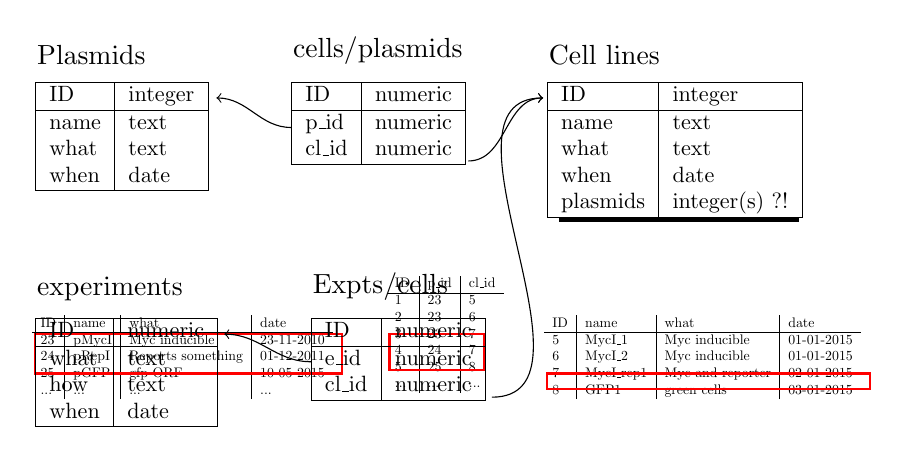
\begin{tikzpicture}[scale=0.5]
%      \draw [help lines, opacity=1] (0,0) grid (22,12);
%      \foreach \x in {1,2,...,20} \node [font=\small] at (\x,0) {\x};
%      \foreach \y in {1,2,...,11} \node [font=\small] at (20,\y) {\y};
      
      \visible<1->{
        \node [below right, align=left, scale=0.8]
        (p1) at (0,11) {
          \begin{tabular}{|l|l|}
            \hline
            ID & integer \\
            \hline
            name & text \\
            what & text \\
            when & date \\
            \hline
          \end{tabular} };
        \node [above right] at (0,11) {Plasmids};
      }
      \visible<2->{
        \node [below right, align=left, scale=0.8]
        (cl1) at (13,11) {
          \begin{tabular}{|l|l|}
            \hline
            ID & integer \\
            \hline
            name & text \\
            what & text \\
            when & date \\
            plasmids & integer(s) ?! \\
            \hline
          \end{tabular} };
        \node [above right] at (13,11) {Cell lines};
      }
      \visible<3->{
        \draw [-, ultra thick] (13.5,7.3) -- (19.6,7.3);
      }

      \visible<4->{
        \node [below right, align=left, scale=0.8]
        (pcl1) at (6.5,11) {
          \begin{tabular}{|l|l|}
            \hline
            ID & numeric \\
            \hline
            p\_id & numeric \\
            cl\_id & numeric \\
            \hline
          \end{tabular} };
        \node [above right ] at (6.5,11) {cells/plasmids};
      }
      \visible<5->{
        \draw [->] (6.7,9.65) to [out=180,in=0]
        (4.8,10.4);
        \draw [->] (11.2,8.8) to [out=0, in=180]
        (13.1,10.4);
      }

      \visible<6-8>{
        \node [below right, align=left, scale=0.5]
        at (0,5) {
          \begin{tabular}{l|l|l|l}
            ID & name & what & date \\
            \hline
            23 & pMycI & Myc inducible & 23-11-2010 \\
            24 & pRepI & Reports something & 01-12-2011 \\
            25 & pGFP & gfp ORF & 10-05-2015 \\
            ... & ... & ... & ...\\
          \end{tabular} };
        
        \node [below right, align=left, scale=0.5]
        at (13,5) {
          \begin{tabular}{l|l|l|l}
            ID & name & what & date \\
            \hline
            5 & MycI\_1 & Myc inducible & 01-01-2015 \\
            6 & MycI\_2 & Myc inducible & 01-01-2015 \\
            7 & MycI\_rep1 & Myc and reporter & 02-01-2015 \\
            8 & GFP1 & green cells & 03-01-2015 \\
          \end{tabular} };
      }
      \visible<7-8>{
        \node [below right, align=left, scale=0.5]
        at (9, 6) {
          \begin{tabular}{l|l|l}
            ID & p\_id & cl\_id \\
            \hline
            1 & 23 & 5 \\
            2 & 23 & 6 \\
            3 & 23 & 7 \\
            4 & 24 & 7 \\
            5 & 25 & 8 \\
            ... & ... & ...\\
          \end{tabular} };
      }
      \visible<8>{
        \draw [red, thick] (9.2,3.5) rectangle (11.6,4.4);
        \draw [red, thick] (0.2,3.4) rectangle (8,4.4);
        \draw [red, thick] (13.2, 3) rectangle (21.4,3.4);
      }
      \visible<9->{
        \node [below right, align=left, scale=0.8]
        (e1) at (0,5) {
          \begin{tabular}{|l|l|}
            \hline
            ID & numeric \\
            \hline
            what & text \\
            how & text \\
            when & date \\
            \hline
          \end{tabular} };
        \node [above right] at (0,5) {experiments};
        \node [below right, align=left, scale=0.8]
        (ecl1) at (7,5) {
          \begin{tabular}{|l|l|}
            \hline
            ID & numeric \\
            \hline
            e\_id & numeric \\
            cl\_id & numeric \\
            \hline
          \end{tabular} };
        \node [above right] at (7,5) {Expts/cells};
        \draw [->] (7.2,3.7) to [out=180,in=0] (5,4.4);
        \draw [->] (11.8,2.8) to [out=0, in=180] (13.1,10.4);
      }
    \end{tikzpicture}
  \end{figure}
\end{frame}

\begin{frame}{virtues}
  grossly oversimplified schema, but:
  \begin{itemize}
  \item We can easily make queries across the data to find things like:
    \begin{itemize}
    \item All cells containing a particular plasmid
    \item All experiments using a cell line containing a plasmid
    \item All experiments / plasmids / experiments made or carried out
      within a given period
    \end{itemize}
  \item Ensure that descriptions of plasmids associated with cell lines
    actually exist (no dangling references).
  \end{itemize}
\end{frame}

\begin{frame}{obvious improvements}
  Include data regarding:
  {\small
  \begin{itemize}
  \item personal identifiers. It is useful to know who made a
    particular reagent or performed an experiment:
    \begin{itemize}
    \item the holder of additional knowledge
    \item to spot trends in data
    \end{itemize}
    $\Rightarrow$ new \texttt{users} table and additional column in relevant tables
  \item plasmid parents? Single column (single main parent) or a plasmid\_parent table
    (multiple parents)
  \item plasmids contain DNA sequences. Can be linked to external genome databases (complex).
  \item Experiment descriptions probably very repetitive. If sufficiently, can be formalised
    to some stupid level of detail.
  \item Sample metadata (experimental details / half way measures etc...) should be included
    as this facilitates automated analyses.
  \item ...
  \end{itemize}
  }
  but there is no end to this, and the database can get infinitely complex.
\end{frame}

\begin{frame}{a confession}
  \pause
  \begin{itemize}
  \item Experiments are very hard to describe formally (too variable!)
    \pause
  \item Creating an interface that doesn't make data entry / modification / 
    lookup a right pain is maybe even more difficult
    \pause
  \item In most cases I would recommend using a collection of notebooks
    rather than spending time with a computer.
  \end{itemize}

  But... there are commercial products that aim to solve this kind of problem, maybe they're OK.
  \pause

  \emph{\bfseries big projects} should formalise their experimental procedures / reagents / data
  in databases.
  
\end{frame}

\end{document}